\documentclass[UTF8]{ctexart}
\usepackage{geometry}
\geometry{a4paper,centering,scale=0.8}
\usepackage{graphicx}
\usepackage[format=hang,font=small,textfont=it]{caption}
\usepackage{amsmath}
\usepackage{amsbsy}
\usepackage{braket}
\newcommand{\beq}{\begin{equation}}
\newcommand{\eeq}{\end{equation}}





\title{\heiti 自旋选择器}
\author{翟耀杰}
\date{\today}

\begin{document}

\maketitle
\section{简介}
自旋选择器最初用于兰姆位移型极化离子源(Lamb Shift Polarized Ion Source, LSPIS)\cite{1969Source},它可以做到仅允许一种核自旋磁量子数的氢(氘)原子保持亚稳态通过。在LSPIS中,首先形成处于$2S_{1/2}$亚稳态的氢(氘)原子束;而后亚稳态原子束穿越自旋选择器,在穿越过程中,只有核自旋磁量子数为特定值的原子可以保持亚稳态,其余原子会迅速跃迁至基态;也就是说在自旋选择器出口,处于亚稳态的原子都有相同的核自旋磁量子数;最后利用亚稳态原子与基态原子电离截面的差异,优先电离亚稳态原子,引出形成极化离子束。
\begin{figure}[ht]
\centering
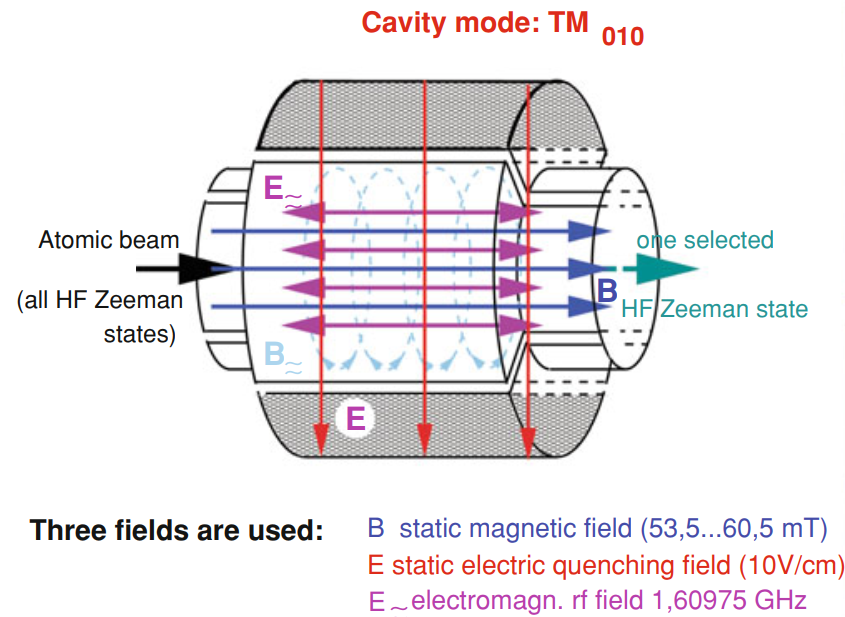
\includegraphics[scale=0.6]{SpinFilterScheme.png}
\caption{自旋选择器示意图}
\label{fig:SFS}
\end{figure}

自旋选择器的示意图如图\ref{fig:SFS},自旋选择功能的实现依赖于其中的纵向静磁场$B$、横向静电场$E_s$,及纵向射频电场$E_{rf}$。可以说,自旋选择器是一个处于静磁场中的圆柱形谐振腔($TM_{010}$模,$1609.75MHz$),腔壁被分割为互相绝缘的四瓣,两组对瓣分别用于施加静电场和射频耦合与采样。对于氢原子而言,自旋选择器静磁场$B=540.8$、$604.4Gs$时分别允许$m_I=1/2$、$-1/2$的氢原子保持亚稳态通过;对于氘原子而言,$B=564.5$、$574.2$、$584.0Gs$时依次分别允许$m_I=1$、$0$、$-1$的氘原子保持亚稳态通过。
\section{物理理论}
在详述自旋选择器物理原理之前,有必要介绍外磁场下氢(氘)原子$n=2$的超精细能级。如图\ref{fig:BRH}所示,在磁场下,考虑超精细相互作用后,氢原子$2S_{1/2}$和$2P_{1/2}$能级分裂成多个磁子能级,图中能级的命名规则沿用Lamb和Rutherford的文献\cite{1950Fine}, 能级名称后的括号内,第一个量子数为电子总角动量磁量子数$m_J$,第二个量子数为核自旋磁量子数$m_I$。氘原子在磁场下的超精细子能级分裂与氢原子相似,依据量子力学角动量叠加的一般法则不难想象,此处不再赘述。
\begin{figure}[ht]
\centering
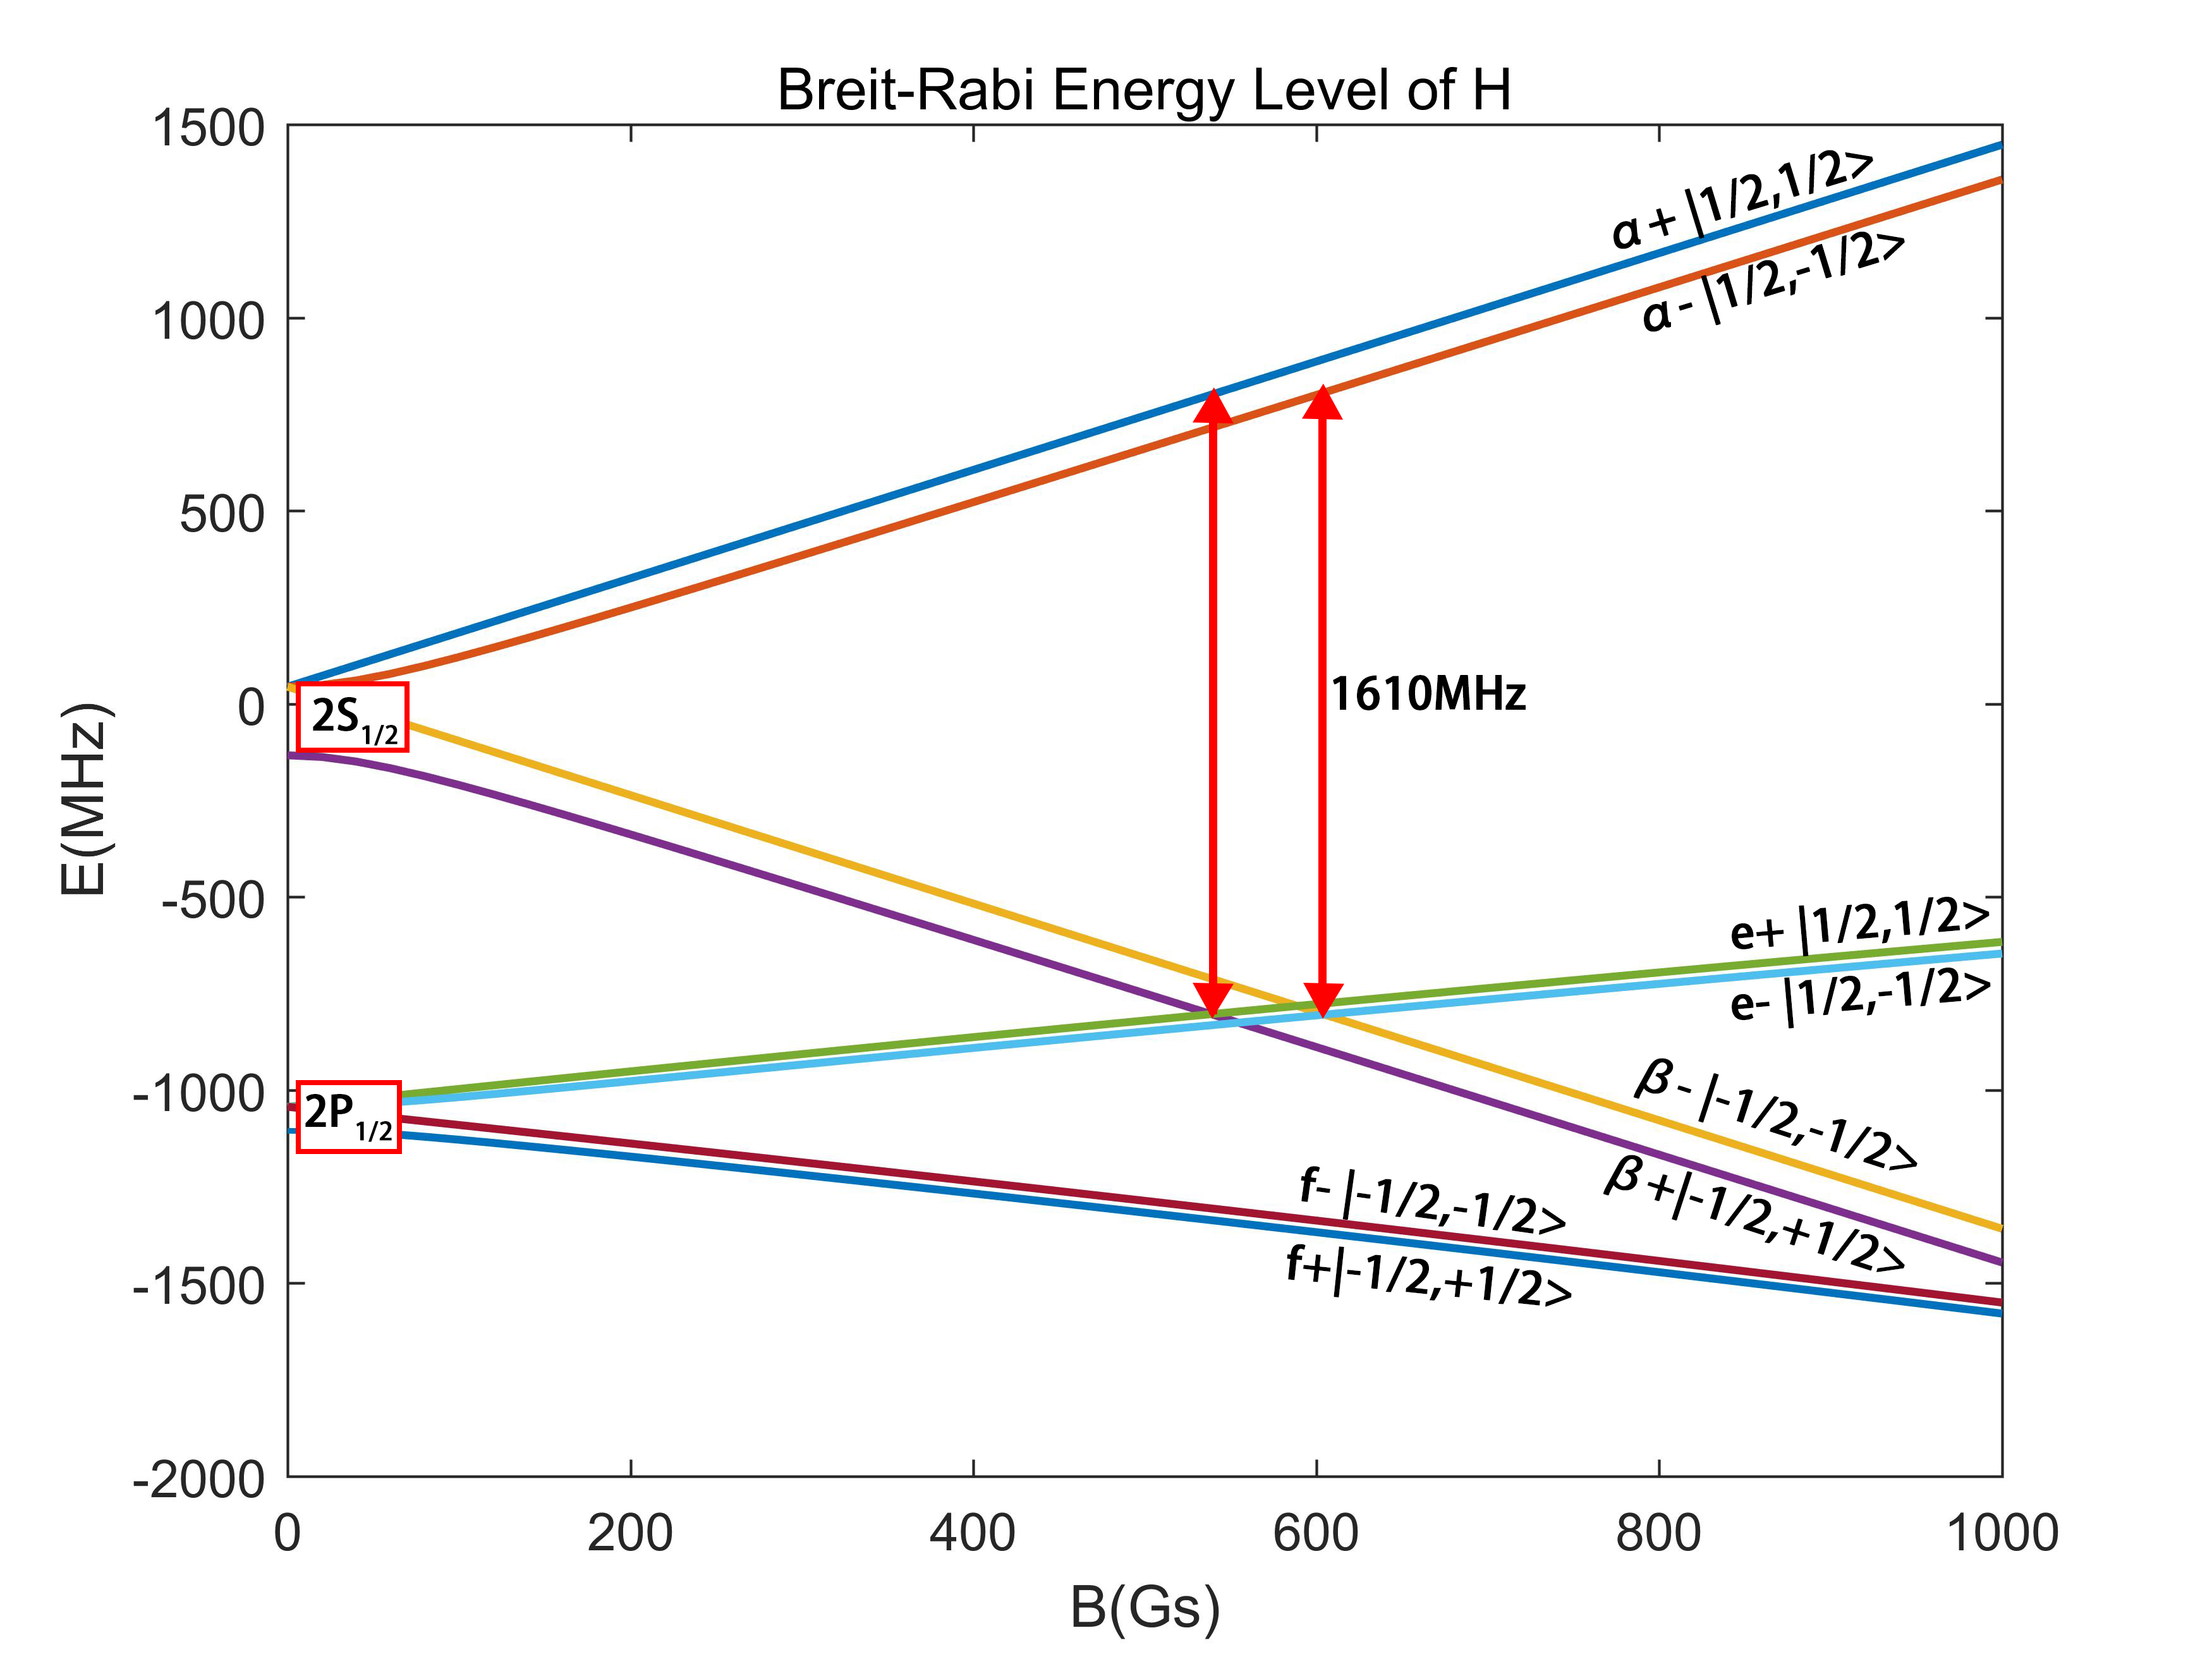
\includegraphics[scale=0.1]{BreitRabiH.jpg}
\caption{氢原子$n=2$磁子能级}
\label{fig:BRH}
\end{figure}

因为自旋选择器工作在强磁场下($500-600Gs$),核自旋磁量子数$m_I$守恒,不同$m_I$能级之间无相互作用,物理分析时可依据$m_I$的不同进行分组考虑,比如,将图\ref{fig:BRH}所示的氢原子$n=2$的各个磁子能级分为$\alpha+$、$\beta+$、$e+$、$f+$及$\alpha-$、$\beta-$、$e-$、$f-$两组进行讨论。在图\ref{fig:BRH}中没有画出$2P_{3/2}$能级,在物理分析对$2P_{3/2}$能级也不予考虑,因为$2P_{3/2}$能级与$2S_{1/2}$、$2P_{1/2}$能级能量差很大,零磁场下,$2P_{3/2}$与$2S_{1/2}$能级差为$9.923GHz$,$2S_{1/2}$与$2P_{1/2}$能级差为$1.049GHz$\cite{EnergyDiff}。自旋选择器为什么可以做到仅允许一种核自旋磁量子数的原子保持亚稳态通过?这实际上是$n=2$氢(氘)原子波函数在外部电磁场下的演化问题。

氢(氘)原子的薛定谔方程可以写为
\beq\label{eq:schrodinger}
(\hat{H}_0+\hat{H}')\psi=i\hbar\frac{\partial\psi}{\partial t}
\eeq
式\eqref{eq:schrodinger}中$\hat{H}_0$是时间独立哈密顿量,包含了外界静磁场$B$与原子磁矩的相互作用,记图\ref{fig:BRH}中所示的各磁子能级波函数为$u_n$,则$\hat{H}_0 u_n=E_n u_n$;$\hat{H}'$是微扰量,包含了静电场$E_s$和射频场$E_rf$、$B_rf$与原子的相互作用。

将波函数$\psi$展开为如下形式
\beq\label{eq:expand}
\psi=\sum a_n(t) u_n e^{-iE_nt/{\hbar}}
\eeq
式\eqref{eq:expand}代入式\eqref{eq:schrodinger}中,两边同乘$u_n^* e^{iE_nt/\hbar}$,化简可得
\beq\label{eq:ampdiff}
i\hbar \dot{a}_k = \sum H'_{kn} a_n e^{i\omega_{kn}t}
\eeq
式\eqref{eq:ampdiff}中$\omega_{kn}=(E_k-E_n)/\hbar$,$H'_{kn}=\bra{u_k}\hat{H}'\ket{u_n}$。依据式\eqref{eq:ampdiff}写出如下方程
\beq\label{eq:matrix4level}
\left( \begin{array}{c}
i\hbar\dot{a}\\i\hbar\dot{b}\\i\hbar\dot{c}\\i\hbar\dot{d}\\ \end{array} \right)
=\left( \begin{array}{cccc}
0 & H'_{\alpha \beta}e^{i\omega_{\alpha \beta}t} & H'_{\alpha e}e^{i\omega_{\alpha e}t} & H'_{\alpha f}e^{i\omega_{\alpha f}t}\\
H'_{\beta \alpha}e^{i\omega_{\beta \alpha}t} & 0 & H'_{\beta e}e^{i\omega_{\beta e}t} & H'_{\beta f}e^{i\omega_{\beta f}t}\\
H'_{e \alpha}e^{i\omega_{e \alpha}t} & H'_{e \beta}e^{i\omega_{e \beta}t} & -i\hbar/\tau & H'_{ef}e^{i\omega_{ef}t}\\
H'_{f \alpha}e^{i\omega_{f \alpha}t} & H'_{f \beta}e^{i\omega_{f \beta}t} & H'_{fe}e^{i\omega_{fe}t} & -i\hbar/\tau\\
\end{array} \right)
\left(\begin{array}{c}
a \\ b \\ c \\ d \\
\end{array} \right)
\eeq
式\eqref{eq:matrix4level}中分别以$a$,$b$,$c$,$d$表示氢(氘)原子处于$\alpha$,$\beta$,$e$,$f$态的概率幅;$\tau$ 为$2P$态平均寿命, $\tau = 1.6ns$。注意式\eqref{eq:matrix4level}并未区分不同核自旋磁量子数$m_I$,前文已经提到由于自旋选择器工作在强磁场下,$m_I$守恒,可对不同$m_I$分组考虑。举例来说,分析$m_I=1/2$的氢原子波函数的演化时,式\eqref{eq:matrix4level}中$\omega_{\alpha \beta}$为$\alpha+$与$\beta+$的能级差,分析$m_I=-1/2$的氢原子波函数的演化时,$\omega_{\alpha \beta}$为$\alpha-$与$\beta-$的能级差。求解方程组\eqref{eq:matrix4level}可得不同$m_I$氢(氘)原子波函数在外部电磁场下的演化情况。下面的重点是求方程组\eqref{eq:matrix4level}中各微扰矩阵元$H'_{kn}$。


\section{模拟计算}

\section{工程分析}

\bibliographystyle{plain}
\bibliography{ref}

\end{document}

